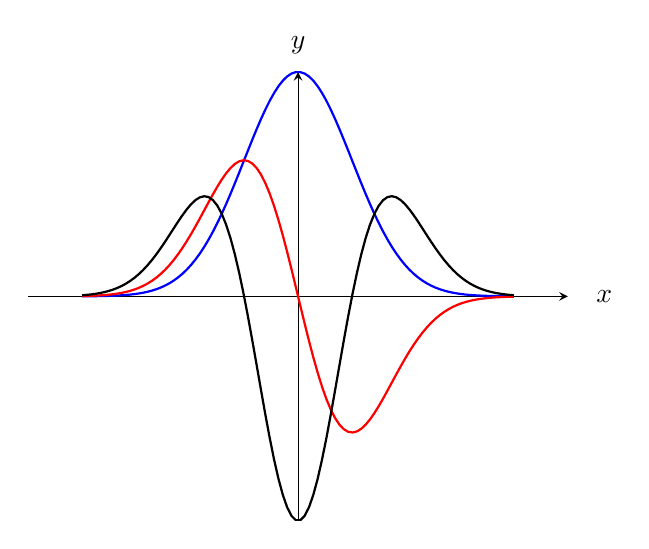
\begin{tikzpicture}
    \begin{axis}[
        axis x line = middle,
        axis y line = middle,
        every axis y label/.style={at={(ticklabel cs:1.1)}},
        y label style={at={(axis description cs:.5,1.1)},anchor=north},
        ylabel = {$y$},
        every axis x label/.style= {at ={(ticklabel cs:1)}},
        x label style={at={(axis description cs:1.1,.5)},anchor=east},
        xlabel = {$x$},
        xmin=-5,xmax=5,
        ymax=1,
        xtick = \empty,
        ytick = \empty
    ]
    \addplot[thick, domain=-4:4, samples=100, color=blue] {exp(-1*x^2/2)};
    \addplot[thick, domain=-4:4, samples=100, color=red] {-x*exp(-x^2/2)};
    \addplot[thick, domain=-4:4, samples=100] {-exp(-x^2/2) +x^2*exp(-x^2/2)};
    \end{axis}
\end{tikzpicture}